\documentclass{article}
\usepackage{maa-monthly}

%% IF YOU HAVE FONTS INSTALLED
%\usepackage{mtpro2}
%\usepackage{mathtime}
\usepackage{subcaption}
%\theoremstyle{theorem}
\usepackage[export]{adjustbox}
\usepackage{hyperref}

\newtheorem{theorem}{Theorem}
\newtheorem{proposition}[theorem]{Proposition}
\newtheorem{lemma}[theorem]{Lemma}
\newtheorem{corollary}[theorem]{Corollary}

\theoremstyle{definition}
\newtheorem*{definition}{Definition}
\newtheorem*{remark}{Remark}

\begin{document}

\title{Flows and the Complex Ackermann Function}
\markright{Complex Ackermann Function}
\author{Author}

\maketitle

\begin{abstract}
The process of extending maps to flows is called continuous or fractional iteration. Extending tetration to the complex numbers is a classic example, finding functional square roots is another.

A general method of fractional iteration in the complex plane is presented based on Faà di Bruno's formula which decomposes the iterations of holomorphic functions into recursive Bell polynomials.

The classical Ackermann function along with fractional iteration defines an Ackermann function for complex numbers. 
\end{abstract}

\noindent

Many mathematicians consider the Euler identity $e^{\pi i}+1=0$ to be beautiful. It is natural to ask what other related beauty exists. The arithmetical operator exponentiation is at the center of the Euler identity. But the \href{https://en.wikipedia.org/wiki/Ackermann_function}{Ackermann function} contains a countable infinite number of \href{https://en.wikipedia.org/wiki/Hyperoperation}{hyperoperators} that succeed exponentiation. 

\section{Derivatives of Iterated Functions}

\subsection{The Zeroth and First Derivative}

Consider the holomorphic function $f(z): \mathbb{C} \rightarrow \mathbb{C}$ and its iterates $f^t(z), t \in \mathbb{N}$ with a fixed point $L\in\mathbb{C}$ such that $f(L)=L$. The first derivative of iterated function $D^nf^t(L)$ is $Df^t(L)=f'(L)^t$, the most important factor in the dynamics of the map.

\subsection{The Second Derivative}
This subsection provides an example of a derivative of an iterated function before presenting the general case. The role of recursion and geometrical series can be seen and will be proven later.

\begin{eqnarray*}
	D^2f(g(z))&=&f''(g(z))g'(z)^2+f'(g(z))g''(z)\\
	        &=&f''(f^{t-1}(z))(Df^{t-1}(z))^2+f'(f^{t-1}(z))D^2f^{t-1}(z)
\end{eqnarray*}


Setting $g(z) = f^{t-1}(z)$ and $z=L$ results in
$$D^2f^t(L) = f''(L) f'(L)^{2t-2}+f'(L) D^2f^{t-1}(L)$$

When $f'(L) \neq 0$, a recurrence equation is formed that is solved as a geometrical series. 
\begin{eqnarray}	           
 D^2f^t(L)&=&f'(L)f''(L)^{2t-2}+f'(L) D^2f^{t-1}(L)\nonumber\\
            &=&f'(L)^0f''(L) f'(L)^{2t-2}\nonumber\\
            &&+f'(L)^1f''(L) f'(L)^{2t-4}\nonumber\\
            &&+\cdots\nonumber\\
            &&+f'(L)^{t-2}f''(L) f'(L)^2\nonumber\\
            &&+f'(L)^{t-1}f''(L) f'(L)^0\nonumber\\
            &=&f''(L)\sum_{k_1=0}^{(t-1)}f'(L)^{2t-k_1-2}
 \label{eq:TheSecondDerivative}            
\end{eqnarray}

\subsection{Recursive Bell Polynomials}

\begin{theorem}[Recursive Bell Polynomial Theorem]
The derivatives of an iterated holomorphic function with a non-superattracting fixed point can be expressed in terms of the geometrical series of recursive Bell polynomials.
$$D^nf^t(L)=\sum_{r=0}^\infty(\sum_{k=2}^n \frac{f^{(k)}(L)}{k!} B_{n,k}(D^2f^{t-1}(L),\ldots, D^{n-k+1}f^{t-1}(L)))^r$$
\end{theorem}

\begin{proof} Consider the following two steps.

\begin{itemize}
\item Recursion:
The following is a version of the Faà di Bruno's formula, \cite{weisstein}

${D^n} f(g(x)) = \sum_{k=1}^n f^{(k)}(g(x))\cdot B_{n,k}\left(g'(x),g''(x),\dots,g^{(n-k+1)}(x)\right)$.

Set $g(x)=f^{t-1}(x)$ and $x=L$,

$D^nf^t(L)=\sum_{k=1}^n \frac{f^{(k)}(L)}{k!} B_{n,k}(Df^{t-1}(L),\ldots, D^{n-k+1}f^{t-1}(L))$

    \item Geometrical series: By strong induction

\end{itemize}

\texttt{\emph{Basis step $n=0$}: $D^0f^{t-1}(L)=L$}.

\texttt{\emph{Inductive step ($0<k<n$):} $D^kf^{t-1}(L)$ is known}.

 $D^nf^{t-1}(L)$ \texttt{is not known but can be solved by a simple recursive expression resulting in the geometrical series where }$C$ \texttt{is independent and can be treated as a constant.}

\texttt{\emph{Inductive Hypothesis}}

$D^nf^t(x)=C+f'(L)D^nf^{t-1}(x)$.

By Taylor series $f^t(x)=\sum_{k=0}^\infty\frac{1}{k!} D^nf^t(L) (x - L)^k$
\end{proof}

\section{Flows}

$$\Phi(0,x) = x$$
$$\Phi(a,\Phi(b,x)) = \Phi(a+b, x),$$

\begin{theorem}[Convergence]

\end{theorem}

\begin{proof}

\end{proof}

\begin{theorem}[Uniqueness]

\end{theorem}

\begin{proof}

\end{proof}

\cite{jackson}

\section{Ackermann Function}
The following is based on the original definition of the Ackermann function where $m,n,p\in\mathbb{N}$. \cite{ackermann}
\begin{align}
\varphi(m, n, 0) &= m + n \\ \nonumber
\varphi(m, 0, 1) &= 0 \\ \nonumber
\varphi(m, 0, 2) &= 1 \\ \nonumber
\varphi(m, 0, p) &= m && \text{for } p > 2 \\ \nonumber
\varphi(m, n, p) &= \varphi(m, \varphi(m, n-1, p), p - 1) && \text{for } n, p > 0 \nonumber
\end{align}

$p\in\mathbb{N}$ and $m,n\in\mathbb{C}$

\begin{align}
\varphi(m, n, 0) &= m + n \\ \nonumber
\varphi(m, 0, 1) &= m\times n \\ \nonumber
\varphi(m, 0, 2) &= m^n \\ \nonumber
\varphi(m, 0, p) &= m && \text{for } p > 2 \\ \nonumber
\varphi(m, n, p) &= \varphi(m, \varphi(m, n-1, p), p - 1) && \text{for } n, p > 0 \nonumber
\end{align}


If $\varphi(m, z, p)$ converges then where $q>p$ the higher hyperoperators $\varphi(m, z, q)$ converge.

\subsection{Convergence}


\begin{figure}[htp]
\centering
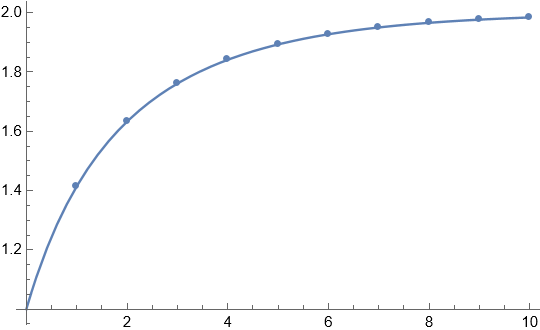
\includegraphics[width=0.5\textwidth]{Ackermann.png}
\caption{Exponential map of $\sqrt{2}^x$ compared with the tetration flow $^x(\sqrt{2})$}
\label{fig:tetration}
\end{figure}

\section{Mathematica code}
\begin{verbatim}
   Flow[f_, t_, x_, L_, order_ : 3] := Module[{s},
   H[0] = L;
   H[1] = f'[L]^t ;
   Do[H[max] = First[r[t] /. 
      RSolve[{r[0] == 0, r[t] ==
        Sum[Derivative[k][f][L] BellY[max, k,Table[H[j]
          /. t -> t - 1, {j, max}]], {k, 2, max}] 
        + f'[L] r[t - 1]}, r[t], t]], 
   {max, 2, order}];
   s = Sum[1/k! H[k] (x - L)^k, {k, 0, order}]
];
\end{verbatim}

\begin{acknowledgment}{Acknowledgment.}
The authors wish to thank the Greek polymath Anonymous, whose prolific works are an endless source of inspiration.
\end{acknowledgment}

\begin{thebibliography}{1}
\bibitem{weisstein} Weisstein, Eric W. "Faà di Bruno's Formula." From 
\textit{MathWorld}--A Wolfram Web Resource. 

\bibitem{jackson} Jackson,E. Atlee  (1995)
\textit{ Perspectives of nonlinear dynamics 1}
Cambridge

\bibitem{ackermann} Ackermann, Wilhelm "Hilbert's construction of the real numbers" (1928).
\textit{From Frege to Gödel}

\end{thebibliography}


\vfill\eject

\end{document}
